\lecture{4}{4. September 2025}{Center of Gravity}

\section{Center of Gravity and Centroid}

\subsection{Center of Gravity and the centroid of a body}
A body can be thought of as consisting of an infinite amount of differential particles (actually bodies consist of discrete atoms, but it is helpful to think of it in the infinite sense). If a body is located in a gravitational field, each of the particles will be subject to a weight $\mathrm{d}W$. These weights will form an approximately parallel system of forces and the resultant of this system is the total weight of the body, which passes through a single point called the center of gravity.

\begin{figure} [ht]
  \centering
  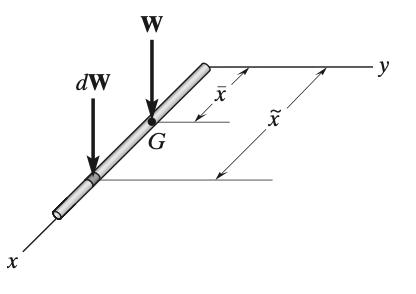
\includegraphics[width=0.5\linewidth]{./figures/f6_1.png}
  \caption{}
  \label{fig:f6_1}
\end{figure}

We consider the rod on \autoref{fig:f6_1}, where the segment with weight $\mathrm{d}W$ is located at an arbitrary position $\tilde{x}$. The total weight of the rod is then:
\[ 
W = \int \, \mathrm{d}W
.\]

The location of the canter of gravity, measured from the $y$-axis is determined by equating the moment of $W$ about the $y$-axis to the sum of the moments of the weights of all its particles about said axis. I.e.
\[ 
\overline{x} W = \int \overline{x} \, \mathrm{d}W \implies \overline{x} = \frac{\int  \overline{x} \, \mathrm{d}W}{\mathrm{d}W}
.\]
This same procedure can be applied for all axes, i.e.
\[ 
\overline{x} = \frac{\int \overline{x}\, \mathrm{d}W}{\int \mathrm{d}W}, \quad \overline{y} = \frac{\int \overline{y} \, \mathrm{d}W}{\int  \mathrm{d}W}, \quad \overline{z} = \frac{\int \overline{z} \, \mathrm{d}W}{\int \, \mathrm{d}W}
.\]


\subsubsection{Centroid of a Volume}
We consider the body on \autoref{fig:f6_2}. If it is made from a homogeneous material, then its specific weight $\gamma$ will be constant. Therefore, a differential element of volume $\mathrm{d}V$ has a weight $\mathrm{d}W = \gamma \, \mathrm{d}V$. Substituting this into the equations from before, and cancelling out $\rho$ we obtain the coordinates of the centroid $C$ as:

\[ 
  \overline{x} = \frac{\int_V \tilde{x} \, \mathrm{d}V}{\int_V \, \mathrm{d}V}, \quad \overline{y} = \frac{\int_V \tilde{y} \, \mathrm{d}V}{\int_V \, \mathrm{d}V}, \quad \overline{z} = \frac{\int_V \tilde{z} \, \mathrm{d}V}{\int_V \, \mathrm{d}V}
.\]

\begin{figure} [ht]
  \centering
  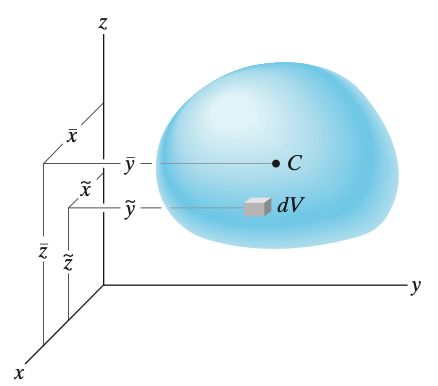
\includegraphics[width=0.5\linewidth]{./figures/f6_2.png}
  \caption{}
  \label{fig:f6_2}
\end{figure}


\subsubsection{Centroid of an area}
Similarly, if an area lies in the $x$-$y$-plane and is bounded by the curve $y = f(x)$ then its centroid will be in the same plane and can be determined as:
\[ 
  \overline{x} = \frac{\int_A \tilde{x} \, \mathrm{d}A}{\int_A \, \mathrm{d}A}, \quad \overline{y} = \frac{\int_A \tilde{y} \, \mathrm{d}A}{\int_A \, \mathrm{d}A}
.\]


\subsection{Composite Bodies}
A composite body consists of a series of connected ``simpler'' bodies. Provided the weight and location of center of gravity of each part we can eliminate the need for integration as:
\[ 
  \overline{x} = \frac{\sum \tilde{x} W}{\sum W}, \quad \overline{y} = \frac{\sum \tilde{y} W}{\sum W}, \quad \overline{z} = \frac{\sum \tilde{z} W}{\sum W}
.\]

